% 图 58.1 —— 由 `checks/emit_hand.py` 自动拼出（probe 精测 + prims2 图元分解）
%%
% ⚠ 这是**稿子不是成品**：跑 `checks/checkhand.py 58.1` 看指标 + 看叠合图。
%%
%% ⚠ 待核：
%   · 本图 probe 报出阴影族 1 个 —— **本脚本不生成阴影**（要照原书手写）；prims2 的 strokes 里可能含阴影线，核对时留意别画重
%   · 可疑字形 1 项（空心圈 ⊙ 常被认成字母 o）—— 见文件末
%%
\documentclass[12pt]{standalone}
\usepackage{fontspec}
\setsansfont{Arial}
\newfontfamily\mfallback{DejaVu Sans}
\usepackage{tikz}
\begin{document}
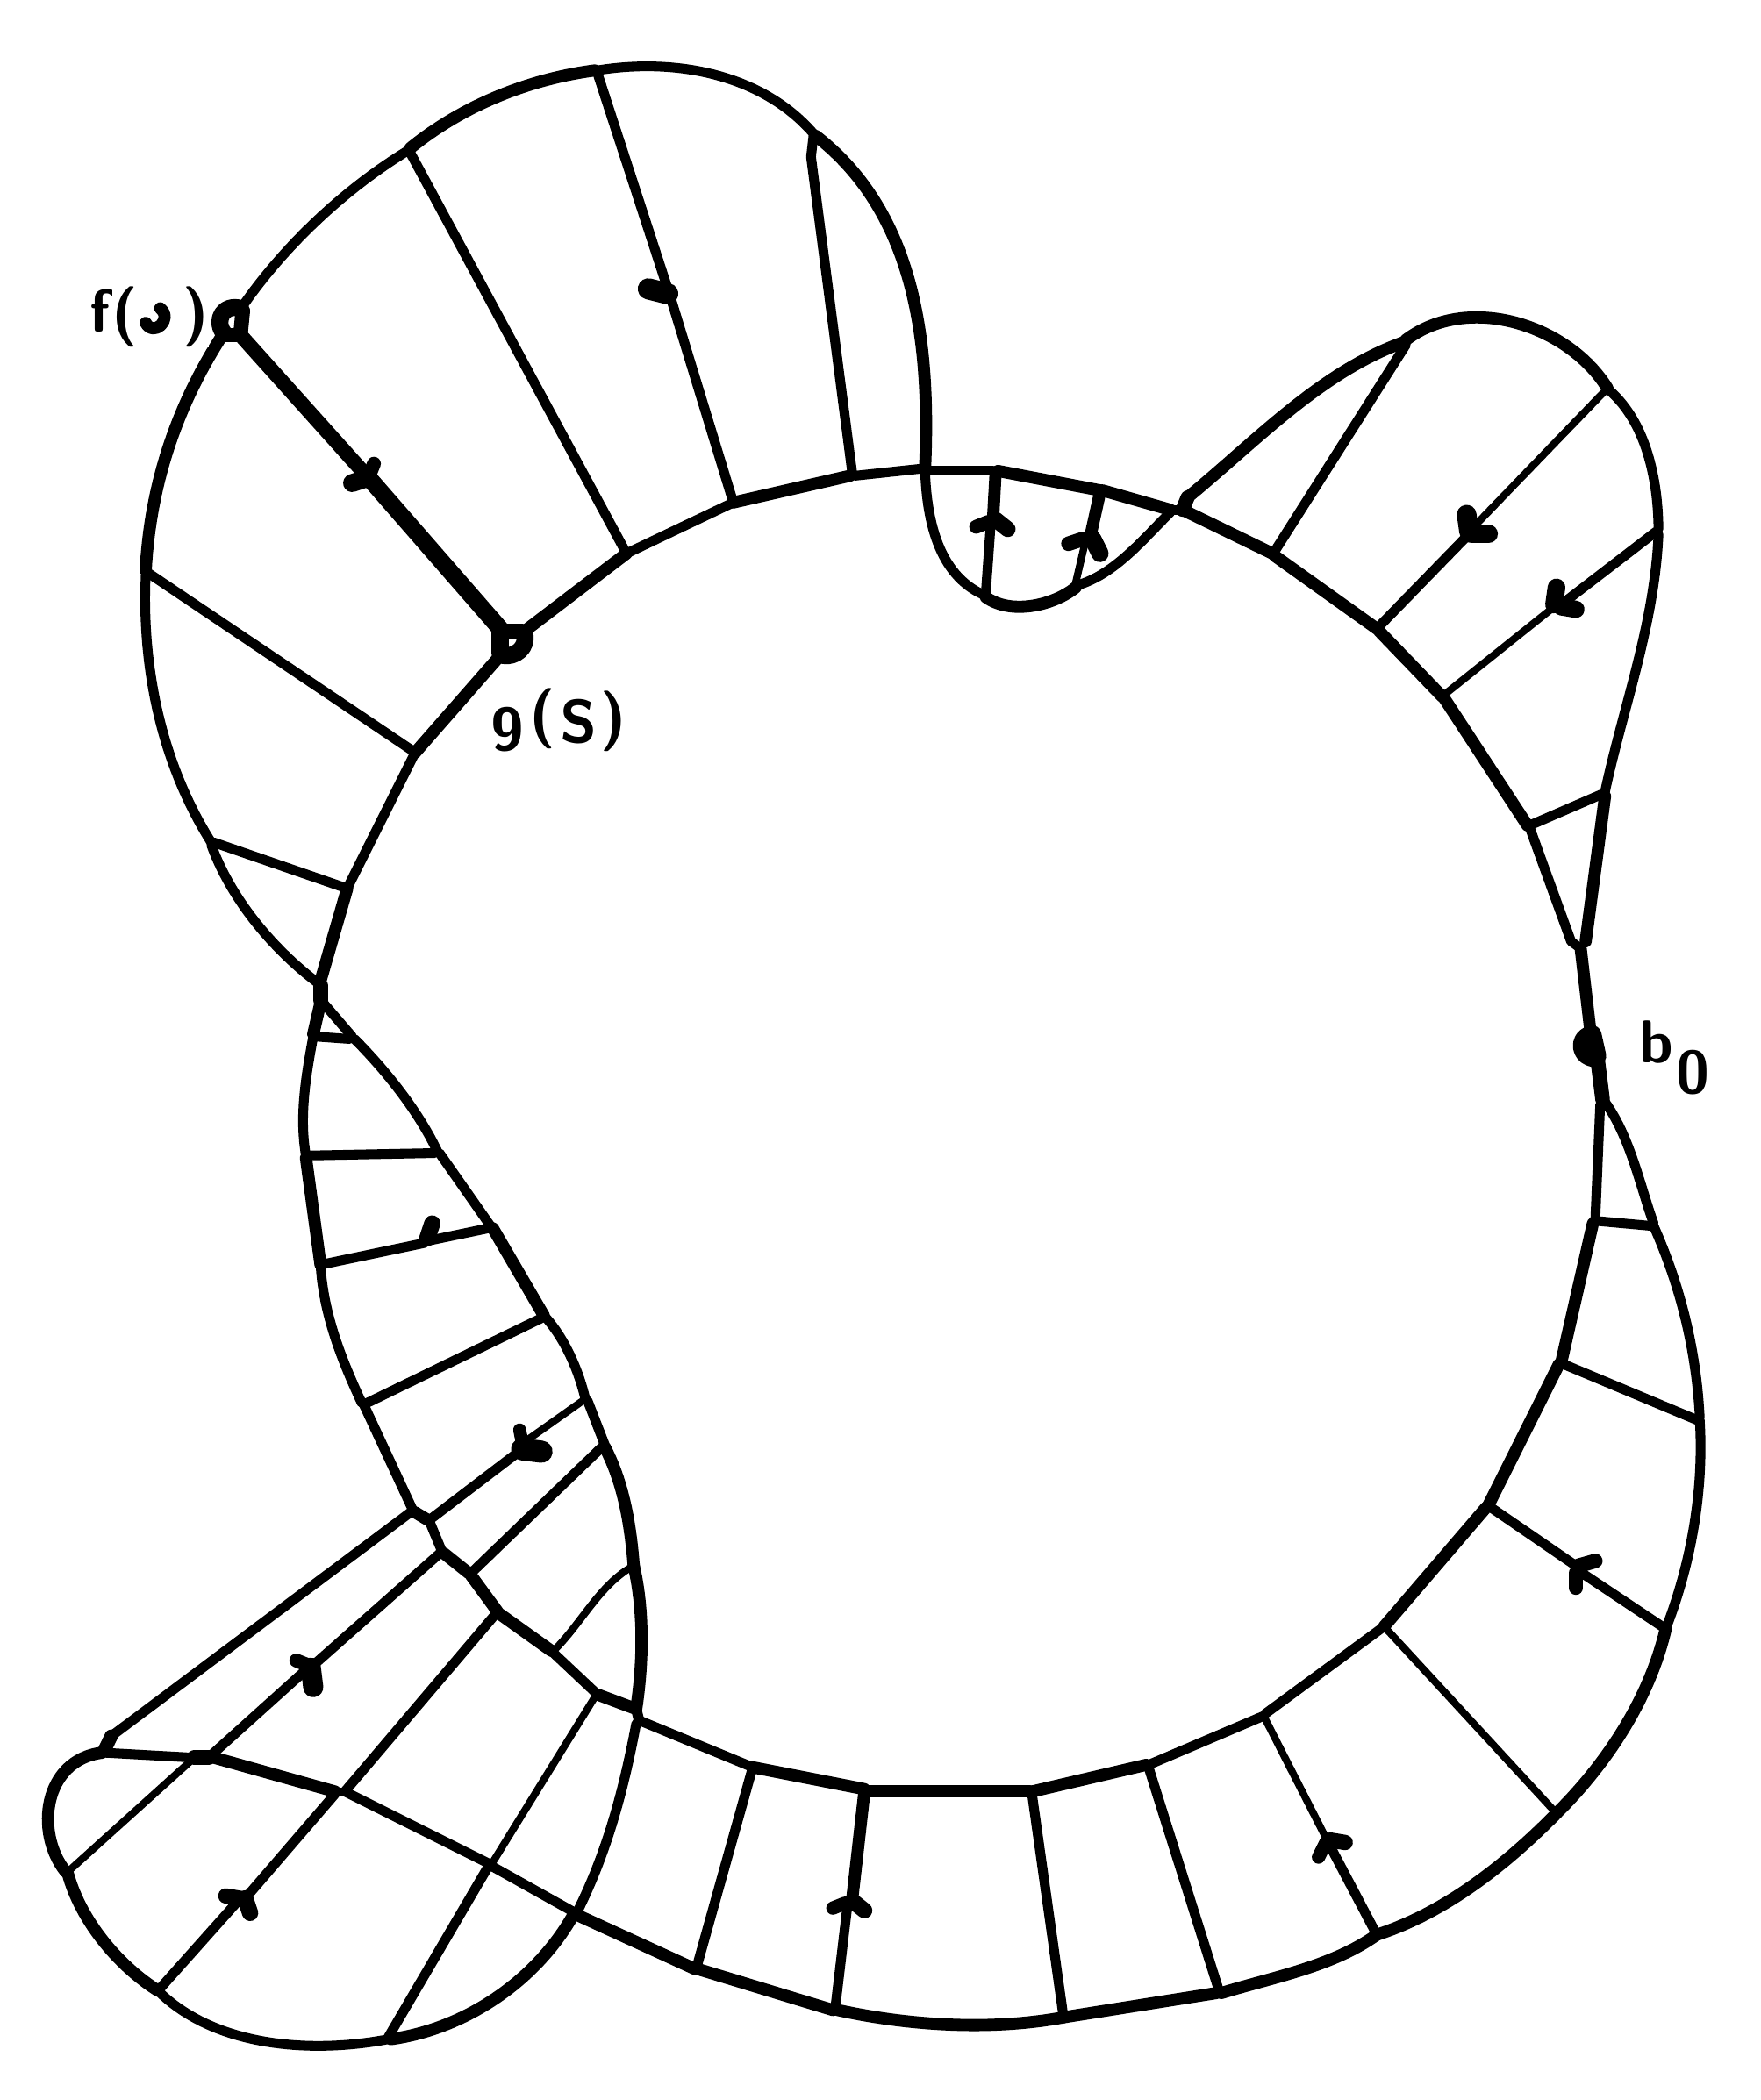
\begin{tikzpicture}[x=1pt, y=-1pt, line width=7.7pt, line cap=round, line join=round]

  %% ════ 直线段（prims2 的 strokes）════
  \draw[line width=7.7pt] (596.0,210.0) -- (603.0,210.0);
  \draw[line width=4.0pt] (634.0,552.0) -- (689.0,575.0);
  \draw[line width=7.1pt] (633.0,240.0) -- (639.0,241.0);
  \draw[line width=5.0pt] (217.0,670.0) -- (196.0,655.0);
  \draw[line width=4.0pt] (569.0,132.0) -- (515.0,217.0);
  \draw[line width=5.0pt] (341.0,772.0) -- (346.0,728.0);
  \draw[line width=3.9pt] (640.0,380.0) -- (637.0,377.8);
  \draw[line width=4.0pt] (637.0,377.8) -- (620.0,331.0);
  \draw[line width=6.0pt] (436.0,212.0) -- (430.0,214.0);
  \draw[line width=4.0pt] (415.0,729.0) -- (428.0,821.0);
  \draw[line width=6.0pt] (90.0,118.0) -- (89.0,128.0);
  \draw[line width=6.3pt] (89.0,772.0) -- (83.0,771.0);
  \draw[line width=4.0pt] (89.0,772.0) -- (56.0,809.0);
  \draw[line width=4.0pt] (117.0,677.0) -- (77.0,713.0);
  \draw[line width=5.0pt] (439.0,211.0) -- (443.0,193.0);
  \draw[line width=5.8pt] (479.1,194.9) -- (477.0,200.0);
  \draw[line width=6.5pt] (400.0,204.0) -- (405.0,208.0);
  \draw[line width=5.0pt] (633.0,551.0) -- (646.0,494.0);
  \draw[line width=5.0pt] (444.0,192.0) -- (472.0,200.0);
  \draw[line width=4.0pt] (232.0,567.0) -- (239.0,585.0);
  \draw[line width=4.0pt] (135.0,417.0) -- (123.0,403.0);
  \draw[line width=5.5pt] (333.0,776.0) -- (338.0,774.0);
  \draw[line width=5.0pt] (414.0,728.0) -- (347.0,728.0);
  \draw[line width=5.0pt] (196.0,260.0) -- (161.0,300.0);
  \draw[line width=4.0pt] (133.0,356.0) -- (78.0,337.0);
  \draw[line width=4.0pt] (133.0,356.0) -- (161.0,300.0);
  \draw[line width=5.0pt] (133.0,356.0) -- (122.0,394.0);
  \draw[line width=7.0pt] (196.0,249.0) -- (142.0,187.0);
  \draw[line width=4.0pt] (51.0,226.0) -- (161.0,300.0);
  \draw[line width=4.0pt] (33.0,712.0) -- (69.0,714.0);
  \draw[line width=3.0pt] (193.0,757.0) -- (235.0,689.0);
  \draw[line width=6.5pt] (341.0,773.0) -- (346.0,777.0);
  \draw[line width=5.0pt] (214.0,532.0) -- (193.0,496.0);
  \draw[line width=5.0pt] (277.0,801.0) -- (333.0,818.0);
  \draw[line width=6.0pt] (122.0,402.0) -- (122.0,396.0);
  \draw[line width=4.0pt] (558.0,248.0) -- (594.0,211.0);
  \draw[line width=5.0pt] (443.0,192.0) -- (401.0,184.0);
  \draw[line width=4.0pt] (265.0,109.0) -- (236.0,20.0);
  \draw[line width=4.0pt] (141.0,568.0) -- (213.0,533.0);
  \draw[line width=7.0pt] (196.0,251.0) -- (196.0,259.0);
  \draw[line width=7.4pt] (135.0,189.0) -- (141.0,187.0);
  \draw[line width=4.0pt] (640.0,637.0) -- (676.0,661.0);
  \draw[line width=7.3pt] (630.0,239.0) -- (631.0,232.0);
  \draw[line width=4.0pt] (192.0,495.0) -- (171.0,465.0);
  \draw[line width=5.0pt] (619.0,330.0) -- (585.0,278.0);
  \draw[line width=4.0pt] (120.0,417.0) -- (134.0,418.0);
  \draw[line width=4.0pt] (169.0,465.0) -- (117.0,466.0);
  \draw[line width=6.0pt] (647.0,633.0) -- (640.0,635.0);
  \draw[line width=3.0pt] (69.0,715.0) -- (18.0,761.0);
  \draw[line width=3.0pt] (511.0,698.0) -- (536.0,747.0);
  \draw[line width=4.0pt] (325.0,46.0) -- (324.0,54.6);
  \draw[line width=4.0pt] (324.0,54.6) -- (341.0,185.0);
  \draw[line width=5.0pt] (584.0,277.0) -- (558.0,250.0);
  \draw[line width=5.0pt] (428.0,821.0) -- (491.0,811.0);
  \draw[line width=5.0pt] (161.0,613.0) -- (166.0,616.0);
  \draw[line width=4.0pt] (119.0,676.0) -- (171.0,630.0);
  \draw[line width=5.0pt] (122.0,511.0) -- (116.0,467.0);
  \draw[line width=4.0pt] (122.0,511.0) -- (165.0,502.0);
  \draw[line width=3.0pt] (129.0,728.0) -- (132.0,728.0);
  \draw[line width=5.0pt] (340.0,186.0) -- (292.0,197.0);
  \draw[line width=5.0pt] (252.0,694.0) -- (236.0,688.0);
  \draw[line width=4.3pt] (252.0,694.0) -- (253.0,698.0);
  \draw[line width=5.0pt] (78.0,714.0) -- (128.0,728.0);
  \draw[line width=5.7pt] (112.0,674.0) -- (117.0,676.0);
  \draw[line width=4.0pt] (604.0,611.0) -- (639.0,635.0);
  \draw[line width=8.1pt] (594.0,202.0) -- (595.0,209.0);
  \draw[line width=5.3pt] (205.0,584.0) -- (204.0,579.0);
  \draw[line width=6.0pt] (83.0,128.0) -- (89.0,128.0);
  \draw[line width=4.0pt] (339.0,775.0) -- (334.0,817.0);
  \draw[line width=4.0pt] (235.0,687.0) -- (218.0,671.0);
  \draw[line width=4.0pt] (167.0,617.0) -- (172.0,629.0);
  \draw[line width=6.7pt] (93.0,778.0) -- (91.0,772.0);
  \draw[line width=3.0pt] (437.0,213.0) -- (433.0,230.0);
  \draw[line width=3.0pt] (596.0,208.0) -- (651.0,151.0);
  \draw[line width=5.0pt] (603.0,610.0) -- (632.0,552.0);
  \draw[line width=4.0pt] (647.0,492.0) -- (649.0,445.0);
  \draw[line width=6.0pt] (648.0,427.0) -- (650.0,443.0);
  \draw[line width=4.0pt] (537.0,749.0) -- (557.0,787.0);
  \draw[line width=6.0pt] (197.0,250.0) -- (205.0,250.0);
  \draw[line width=5.0pt] (206.0,250.0) -- (248.0,218.0);
  \draw[line width=4.0pt] (227.0,778.0) -- (193.0,759.0);
  \draw[line width=4.0pt] (205.0,587.0) -- (167.0,616.0);
  \draw[line width=9.1pt] (205.0,587.0) -- (213.0,588.0);
  \draw[line width=5.0pt] (514.0,218.0) -- (477.0,200.0);
  \draw[line width=7.1pt] (440.0,212.0) -- (443.0,218.0);
  \draw[line width=4.0pt] (670.0,495.0) -- (648.0,493.0);
  \draw[line width=4.0pt] (463.0,717.0) -- (510.0,697.0);
  \draw[line width=4.0pt] (191.0,759.0) -- (150.0,829.0);
  \draw[line width=6.0pt] (76.0,714.0) -- (70.0,714.0);
  \draw[line width=4.0pt] (184.0,638.0) -- (238.0,586.0);
  \draw[line width=4.0pt] (159.0,53.0) -- (248.0,218.0);
  \draw[line width=4.0pt] (672.0,209.0) -- (633.0,239.0);
  \draw[line width=5.5pt] (536.0,749.0) -- (533.0,755.0);
  \draw[line width=4.0pt] (511.0,696.0) -- (560.0,660.0);
  \draw[line width=5.0pt] (346.0,727.0) -- (300.0,718.0);
  \draw[line width=4.0pt] (292.0,197.0) -- (266.0,112.0);
  \draw[line width=4.0pt] (292.0,197.0) -- (248.0,218.0);
  \draw[line width=4.0pt] (492.0,810.0) -- (463.0,718.0);
  \draw[line width=5.0pt] (645.0,415.0) -- (641.0,381.0);
  \draw[line width=5.0pt] (276.0,801.0) -- (228.0,779.0);
  \draw[line width=3.0pt] (585.0,276.0) -- (630.0,240.0);
  \draw[line width=5.0pt] (122.0,403.0) -- (119.0,416.0);
  \draw[line width=3.0pt] (230.0,567.0) -- (206.0,584.0);
  \draw[line width=4.0pt] (91.0,772.0) -- (128.0,729.0);
  \draw[line width=5.7pt] (144.0,181.0) -- (142.0,186.0);
  \draw[line width=4.0pt] (140.0,569.0) -- (160.0,612.0);
  \draw[line width=4.0pt] (370.0,183.0) -- (342.0,186.0);
  \draw[line width=4.0pt] (192.0,758.0) -- (132.0,728.0);
  \draw[line width=4.0pt] (194.0,655.0) -- (132.0,728.0);
  \draw[line width=4.0pt] (254.0,699.0) -- (300.0,718.0);
  \draw[line width=3.0pt] (641.0,380.0) -- (643.0,377.8);
  \draw[line width=5.0pt] (643.0,377.8) -- (651.0,318.0);
  \draw[line width=3.0pt] (631.0,737.0) -- (560.0,660.0);
  \draw[line width=5.0pt] (557.0,249.0) -- (515.0,219.0);
  \draw[line width=6.7pt] (166.0,500.0) -- (168.0,494.0);
  \draw[line width=7.0pt] (648.0,425.0) -- (646.0,416.0);
  \draw[line width=6.0pt] (639.0,638.0) -- (639.0,644.0);
  \draw[line width=5.0pt] (415.0,728.0) -- (462.0,717.0);
  \draw[line width=4.0pt] (159.0,613.0) -- (35.8,705.2);
  \draw[line width=5.5pt] (35.8,705.2) -- (33.0,711.0);
  \draw[line width=4.0pt] (277.0,800.0) -- (300.0,718.0);
  \draw[line width=5.0pt] (400.0,185.0) -- (399.0,203.0);
  \draw[line width=4.0pt] (396.0,234.0) -- (398.0,206.0);
  \draw[line width=4.0pt] (650.0,317.0) -- (620.0,330.0);
  \draw[line width=5.0pt] (602.0,611.0) -- (560.0,660.0);
  \draw[line width=8.7pt] (257.0,109.0) -- (265.0,111.0);
  \draw[line width=5.7pt] (392.0,207.0) -- (397.0,205.0);
  \draw[line width=5.0pt] (184.0,639.0) -- (195.0,654.0);
  \draw[line width=4.0pt] (372.0,184.0) -- (399.0,184.0);
  \draw[line width=5.0pt] (183.0,638.0) -- (173.0,630.0);
  \draw[line width=6.3pt] (544.0,749.0) -- (538.0,748.0);
  \draw[line width=6.0pt] (89.0,128.0) -- (141.0,186.0);
  \draw[line width=8.3pt] (119.0,685.0) -- (118.0,677.0);
  \draw[line width=4.0pt] (473.0,200.0) -- (477.0,200.0);
  \draw[line width=4.0pt] (167.0,501.0) -- (191.0,496.0);

  %% ════ 曲线（prims2 的 curves —— 三段式，坐标同为 (y,x)）════
  \draw[line width=5.0pt] (251.0,635.0) .. controls (249.6,617.9) and (246.8,600.8) .. (239.0,586.0);
  \draw[line width=3.0pt] (251.0,635.0) .. controls (237.0,642.5) and (229.4,658.9) .. (218.0,670.0);
  \draw[line width=5.0pt] (251.0,635.0) .. controls (255.3,653.5) and (254.9,675.1) .. (252.0,694.0);
  \draw[line width=7.0pt] (197.0,260.0) .. controls (202.2,261.0) and (207.6,256.6) .. (206.0,251.0);
  \draw[line width=4.0pt] (651.0,444.0) .. controls (661.2,458.2) and (665.1,477.3) .. (671.0,494.0);
  \draw[line width=4.0pt] (231.0,566.0) .. controls (228.2,554.3) and (222.7,541.8) .. (215.0,533.0);
  \draw[line width=5.0pt] (568.0,131.0) .. controls (534.1,143.1) and (507.4,171.6) .. (479.1,194.9);
  \draw[line width=4.0pt] (653.0,151.0) .. controls (667.9,164.2) and (672.8,187.4) .. (673.0,208.0);
  \draw[line width=4.0pt] (136.0,418.0) .. controls (149.0,431.1) and (162.1,447.5) .. (170.0,464.0);
  \draw[line width=5.0pt] (335.0,818.0) .. controls (364.3,824.4) and (397.8,826.6) .. (428.0,821.0);
  \draw[line width=4.0pt] (158.0,52.0) .. controls (132.1,67.8) and (107.4,90.9) .. (90.0,116.0);
  \draw[line width=5.0pt] (371.0,182.0) .. controls (373.1,131.8) and (367.2,77.9) .. (326.0,46.0);
  \draw[line width=5.0pt] (226.0,779.0) .. controls (210.4,806.5) and (181.2,825.8) .. (151.0,830.0);
  \draw[line width=4.0pt] (116.0,466.0) .. controls (113.1,449.8) and (116.1,432.5) .. (119.0,417.0);
  \draw[line width=4.0pt] (395.0,235.0) .. controls (376.2,226.6) and (371.8,203.7) .. (371.0,185.0);
  \draw[line width=4.0pt] (236.0,19.0) .. controls (267.5,13.8) and (303.5,20.2) .. (325.0,45.0);
  \draw[line width=4.0pt] (56.0,811.0) .. controls (79.6,833.4) and (118.7,836.0) .. (150.0,830.0);
  \draw[line width=5.0pt] (32.0,712.0) .. controls (8.0,715.0) and (4.1,744.7) .. (17.0,761.0);
  \draw[line width=4.0pt] (122.0,511.0) .. controls (123.2,531.4) and (130.6,549.9) .. (139.0,568.0);
  \draw[line width=5.0pt] (55.0,810.0) .. controls (38.1,799.2) and (23.3,781.0) .. (18.0,762.0);
  \draw[line width=4.0pt] (673.0,210.0) .. controls (671.4,247.1) and (658.6,280.8) .. (651.0,316.0);
  \draw[line width=4.0pt] (690.0,574.0) .. controls (688.6,546.2) and (682.0,519.6) .. (671.0,495.0);
  \draw[line width=4.0pt] (472.0,201.0) .. controls (460.7,212.2) and (449.2,226.4) .. (434.0,231.0);
  \draw[line width=7.0pt] (647.0,426.0) .. controls (640.9,426.3) and (638.8,418.0) .. (645.0,416.0);
  \draw[line width=5.0pt] (493.0,811.0) .. controls (514.5,804.4) and (538.7,800.1) .. (557.0,787.0);
  \draw[line width=5.0pt] (396.0,236.0) .. controls (405.9,243.2) and (423.3,239.8) .. (433.0,232.0);
  \draw[line width=4.0pt] (50.0,227.0) .. controls (48.3,265.6) and (56.7,304.8) .. (77.0,337.0);
  \draw[line width=4.0pt] (252.0,700.0) .. controls (247.0,726.6) and (240.1,752.7) .. (228.0,777.0);
  \draw[line width=5.0pt] (50.0,123.0) .. controls (53.2,129.0) and (61.4,121.6) .. (56.0,117.0);
  \draw[line width=5.0pt] (235.0,19.0) .. controls (207.6,22.6) and (180.5,33.5) .. (159.0,51.0);
  \draw[line width=5.0pt] (631.0,737.0) .. controls (652.1,716.1) and (669.3,689.5) .. (676.0,661.0);
  \draw[line width=5.0pt] (631.0,737.0) .. controls (609.9,758.4) and (585.1,777.9) .. (557.0,787.0);
  \draw[line width=4.0pt] (77.0,338.0) .. controls (85.0,360.0) and (101.8,380.5) .. (121.0,395.0);
  \draw[line width=5.0pt] (569.0,130.0) .. controls (594.9,110.5) and (636.1,124.0) .. (652.0,150.0);
  \draw[line width=4.0pt] (690.0,575.0) .. controls (691.8,604.3) and (686.3,634.6) .. (676.0,661.0);
  \draw[line width=5.0pt] (50.0,225.0) .. controls (51.8,190.4) and (62.4,158.1) .. (81.0,129.0);
  \draw[line width=7.0pt] (89.0,117.0) .. controls (82.0,115.1) and (78.3,121.8) .. (82.0,127.0);

  %% ════ 标签（probe 直接给的 \node 行）════
  %% ⚠ 全部补了 fill=white：文字在最上层，否则与曲线交叉干扰
     \node[anchor=center,inner sep=0pt,fill=white,font=\fontsize{29.1}{36.4}\selectfont] at (32.0,118.0) {\textsf{\textbf{\textit{f}}}};   % box(26,106,11,23)
     \node[anchor=center,inner sep=0pt,fill=white,font=\fontsize{30.7}{38.4}\selectfont] at (41.5,120.5) {\textsf{\textbf{(}}};   % box(37,106,8,28)
     \node[anchor=center,inner sep=0pt,fill=white,font=\fontsize{29.6}{37.0}\selectfont] at (70.5,120.5) {\textsf{\textbf{)}}};   % box(65,107,8,26)
     \node[anchor=center,inner sep=0pt,fill=white,font=\fontsize{31.3}{39.1}\selectfont] at (213.5,286.0) {\textsf{\textbf{(}}};   % box(209,271,8,29)
     \node[anchor=center,inner sep=0pt,fill=white,font=\fontsize{30.2}{37.7}\selectfont] at (242.5,287.0) {\textsf{\textbf{)}}};   % box(237,273,8,27)
     \node[anchor=center,inner sep=0pt,fill=white,font=\fontsize{34.8}{43.5}\selectfont] at (199.0,290.4) {\textsf{\textbf{9}}};   % box(188,278,18,23)
     \node[anchor=center,inner sep=0pt,fill=white,font=\fontsize{24.1}{30.1}\selectfont] at (228.3,287.1) {\textsf{\textbf{\textit{S}}}};   % box(221,278,15,17)
     \node[anchor=center,inner sep=0pt,fill=white,font=\fontsize{29.1}{36.4}\selectfont] at (672.2,419.2) {\textsf{\textbf{\textit{b}}}};   % box(663,407,16,22)
     \node[anchor=center,inner sep=0pt,fill=white,font=\fontsize{24.9}{31.1}\selectfont] at (687.1,431.7) {\textsf{\textbf{0}}};   % box(679,423,12,17)

  % 钉死画布：否则超出的图元/控制点会把页面撑大，1:1 回比就失准
  \pgfresetboundingbox
  \path[use as bounding box] (0,0) rectangle (705,845);
\end{tikzpicture}
\end{document}

% ⚠ 待核清单（probe 拿不准，人眼过一遍）：
%   · 未识别/跳过：⑤ 跳过/未识别的字形
